% -*- mode: LaTeX; coding: utf-8; -*-

\documentclass[a4paper,12pt]{article}

\usepackage{cmap}                   % правильный PDF (на первом месте)
\usepackage{ucs}                    % unicode
\usepackage[utf8x]{inputenc}
\usepackage{mathtext}               % перед загрузкой пакета babel
\usepackage[russian]{babel}
\usepackage[pdftex]{graphicx}       % pdf
\usepackage{indentfirst}            % правильный отступ

\graphicspath{{pictures/}}
\pdfinfo{
  /Author (Jan Musinsky)
  /Title (Drift chambers on STRELA)
  /Subject (Drift chambers)
  /Keywords (Detectors; Drift chambers; STRELA; autocalibration)
}

\begin{document}

% -*- mode: LaTeX; coding: utf-8; -*-

\thispagestyle{empty} \setcounter{page}{0}

\vspace*{8cm} \noindent
{\large
  В. В.~Глаголев$^{1}$, Д. А.~Кириллов${^1}$, Г.~Мартинска$^{2}$,\\
  Я.~Мушински$^{1,2,*}$, Н. М.~Пискунов$^{1}$, Й.~Урбан$^{2}$
}

\vspace{2cm} \noindent
{\large
  ПОИСК И РЕКОНСТРУКЦИЯ ТРЕКА В ДРЕЙФОВЫХ КАМЕРАХ НА УСТАНОВКЕ СТРЕЛА
}

\vspace{4cm} \noindent
{\small
  $^{1}$Объединенный Институт Ядерных Исследований, Дубна\\
  $^{2}$Университет им.~П.~Й.~Шафарика, Кошице, Словакия\\
  $^{*}$E-mail: mucha@sunhe.jinr.ru
}



%%% Local Variables:
%%% mode: latex
%%% TeX-master: "preprint"
%%% End:

\clearpage % -*- mode: LaTeX; coding: utf-8; -*-

\vspace* {2.5cm}
\begin{center} \bf{ВВЕДЕНИЕ} \end{center}

Экспериментальная установка СТРЕЛА предназначена для исследования
зарядово-обменных процессов во взаимодействиях дейтронов с~протонами
\cite{cejp:2008}. Выбор дрейфовых камер в качестве координатных детекторов
спектрометра обусловлен возможностью получения высокого пространственного
разрешения и более надёжного отбора двух близко проходящих треков.

Применение дрейфовых камер требует нахождение соотношения между измеренным
временем дрейфа проходящей частицы и его преобразованием в расстояние
относительно данной сигнальной проволочки. Сначала используется
"<интегральное"> преобразование, после чего происходит поиск и реконструкция
трека. Для получения более корректного соотношения между временем дрейфа
и расстоянием используется итеративная процедура автокалибровки.

\begin{figure}[h]
  \begin{center}
    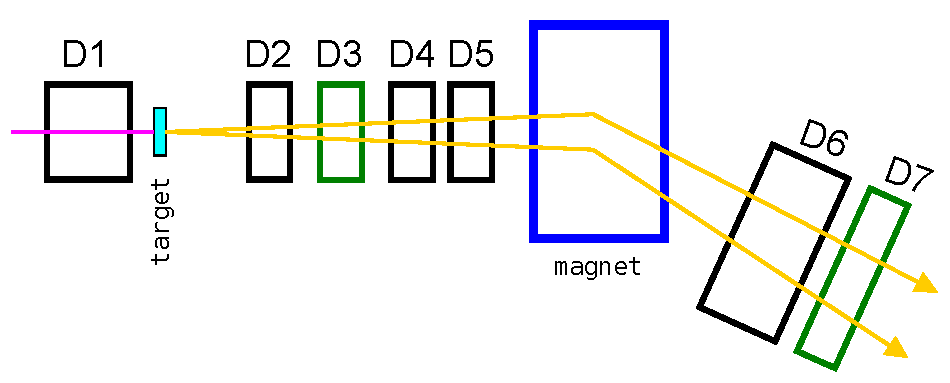
\includegraphics[angle=0,width=13.7cm]{schema.pdf}
    \caption {Схема блоков дрейфовых камер на установке СТРЕЛА.}
    \label{fig:schema}
  \end{center}
\end{figure}

Установка СТРЕЛА \cite{strela:web} представляет одноплечевой спектрометр,
основными элементами которого являются сцинтилляционные счётчики, дрейфовые
камеры и анализирующий магнит. На рис.~\ref{fig:schema} приведена схема
расположения дрейфовых камер на выведенном пучке дейтронов из ускорительного
комплекса Нуклотрона.

В настоящее время используется 7 блоков дрейфовых камер. Конструкция и
характеристики дрейфовых камер изложены в работах \cite{filatova:1977,
  vodopianov:1975, vodopianov:1983}. Сигнальные проволочки (нити) в соседних
слоях сдвинуты относительно друг друга на 21~мм. Такое расположение нитей
позволяет устранить лево-правую неоднозначность в определении пространственных
координат треков частиц. Длина дрейфового промежутка во всех камерах равна
21~мм.

В таблице~\ref{tab:config} приведена структура блоков дрейфовых камер,
регистрируемая координата (ось Z направлена по направлению пучка дейтронов)
количество сигнальных проволочек в каждой плоскости (штриховая координата
используется для сдвинутых проволочек).

\begin{table}[h]
  \begin{center}
    \resizebox{14cm}{!} {
      \begin{tabular}{|l|c|c|c|c|c|c|c|c|c|c|c|c|c|c|c|c|}
        \hline
        расположение блока & \multicolumn{16}{|c|}{до мишени} \\
        \hline
        номер блока & \multicolumn{4}{|c|}{} &
        \multicolumn{8}{|c|}{1} & \multicolumn{4}{|c|}{} \\
        % \hline
        координата & \multicolumn{4}{|c|}{} &
        Y & Y' & Y & Y' & X & X' & X & X' & \multicolumn{4}{|c|}{} \\
        число проволочек & \multicolumn{4}{|c|}{} &
        4 & 3 & 4 & 3 & 4 & 3 & 4 & 3 & \multicolumn{4}{|c|}{} \\
        \hline \hline

        расположение блока & \multicolumn{16}{|c|}{за мишенью} \\
        \hline
        номер блока & \multicolumn{4}{|c|}{2} & \multicolumn{4}{|c|}{3} &
        \multicolumn{4}{|c|}{4} & \multicolumn{4}{|c|}{5} \\
        % \hline
        координата &
        Y & Y' & X & X' & U & U' & V & V' & X & X' & X & X' & Y & Y' & X & X' \\
        число проволочек &
        4 & 3 & 4 & 3 & 4 & 3 & 4 & 3 & 4 & 4 & 3 & 3 & 4 & 3 & 4 & 3 \\
        \hline \hline

        расположение блока & \multicolumn{16}{|c|}{за магнитом} \\
        \hline
        номер блока & \multicolumn{2}{|c|}{} & \multicolumn{8}{|c|}{6} &
        \multicolumn{4}{|c|}{7} & \multicolumn{2}{|c|}{} \\
        % \hline
        координата & \multicolumn{2}{|c|}{} &
        Y & Y' & Y & Y' & X & X' & X & X' & U & U' & V & V' &
        \multicolumn{2}{|c|}{} \\
        число проволочек & \multicolumn{2}{|c|}{} &
        7 & 6 & 7 & 6 & 7 & 6 & 7 & 6 & 7 & 6 & 7 & 6 &
        \multicolumn{2}{|c|}{} \\
        \hline
      \end{tabular}
    }
    \caption{Конфигурация дрейфовых камер на установке СТРЕЛА}
    \label{tab:config}
  \end{center}
\end{table}

До мишени располагается первый блок дрейфовых камер (D1) с размером рабочей
области 125х125 мм$^{2}$, имеющий 4 плоскости Y-координат и 4 плоскости
X-координат. Количество вещества в этом блоке равно 0.141 г/см$^{2}$ (0.008
радиационной длины) \cite{filatova:1977}. Первый блок служит для определения
треков пучковых дейтронов, падающих на мишень.

За мишенью располагаются 4 блока дрейфовых камер с такими же размерами. Первый
блок (D2) имеет 2 плоскости Y-координат и 2 плоскости X-координат, затем блок
(D3) из 2 плоскостей U-координат и 2 плоскостей V-координат. UV координаты
повёрнуты на 22.5 градуса относительно XY координат вокруг оси Z, проходящей
через центры блоков камер в направлении падающего пучка. Далее следует блок
дрейфовых камер (D4) с 4 плоскостями Х-координат и последний блок (D5) имеет
2 плоскости Y-координат и 2 плоскости Х-координат. Такой набор камер после
мишени позволяет надёжно идентифицировать два близко проходящих трека.

За анализирующим магнитом располагаются 2 блока дрейфовых камер размером
250х250 мм$^{2}$, первый (D6) имеет 4 плоскости Y-координат и 4 плоскости
Х-координат, а второй блок (D7) 2 плоскости U-координат и 2 плоскости
V-координат (повёрнутых тоже на 22.5 градуса).

Число всех регистрируемых сигналов с проволочек составляет 162, которые
поступают на входы модулей TDC с временным разрешением 100 пикосекунд.
На камере установлены платы
с 2 микросхемами ASD-8, в которых осуществляется усиление, формирование
и дискриминация входных сигналов от сигнальных проволочек дрейфовых камер.
Такие же платы использовались в системе дрейфовых камер в детекторе
Outer Tracker установки HERA-B \cite{hera:web}.

\vspace* {0.5cm}
\begin{center} \bf{ВРЕМЯ ДРЕЙФА} \end{center}

Изучение характеристик дрейфовых камер было проведено при облучении
полиэтиленовой мишени пучком дейтронов с импульсом 3.5 ГэВ/с на канале 4В
ускорительного комплекса Нуклотрона ЛФВЭ ОИЯИ. Интенсивность пучка была порядка
$\sim$ 5$\times$10$^{5}$ с$^{-1}$. Для получения пучка дейтронов интенсивностью
не более 10$^{5}$ -- 10$^{6}$ с$^{-1}$ использовался стальной коллиматор сечением
4х4~мм$^{2}$ и длиной 1.2~м устанавливаемый в~фокусе Ф3 перед поворотным
магнитом канала ВП~1.

\begin{figure}[h]
  \begin{center}
    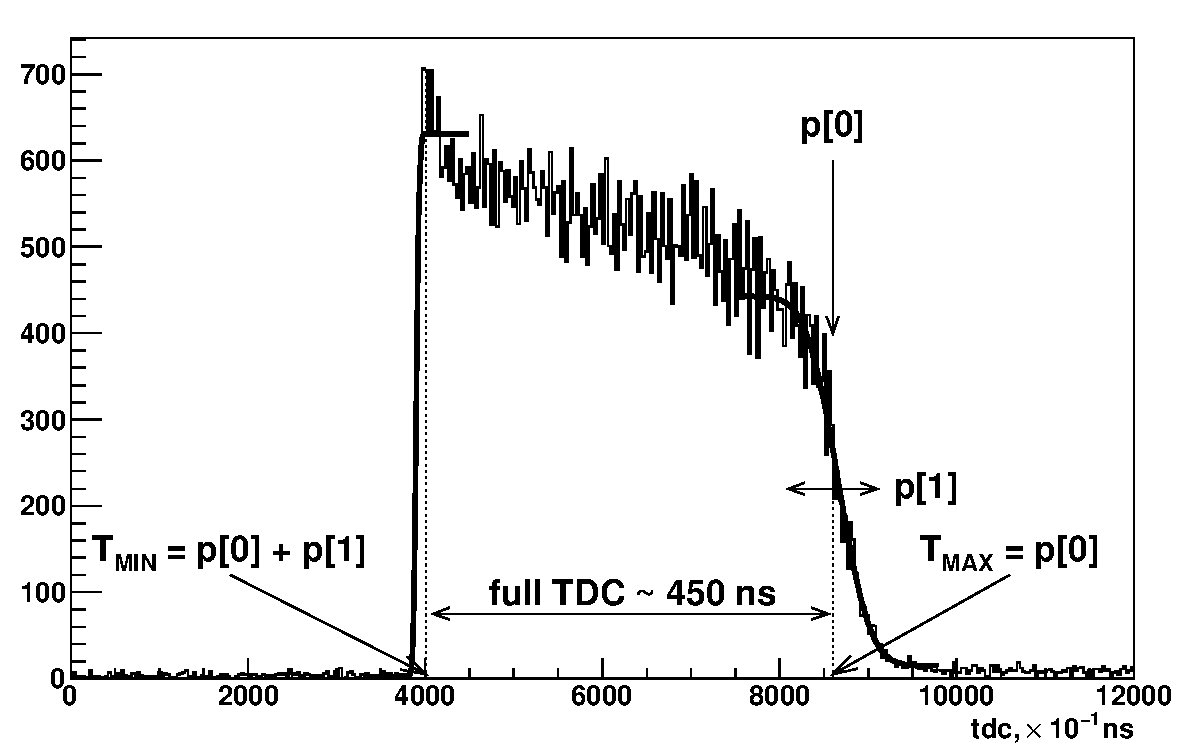
\includegraphics[angle=0,width=12.0cm]{tdc.pdf}
    \caption {Временной спектр TDC одной проволочки дрейфовой камеры.}
    \label{fig:tdc}
  \end{center}
\end{figure}

Блоки камер продувались газовой смесью аргон (72\%) + изобутан (25\%) +
этиловый спирт (3\%). Потенциал катодов распределён равномерно от $-3$ кВ до 0
и обеспечивает напряжённость поля $\sim$ 1.5 кВ/см вдоль дрейфа электронов.
На сигнальную проволочку подаётся положительный потенциал $+$1.65 кВ,
на потенциальную $-$3.0 кВ.

Временной спектр TDC одного из каналов показан на рис.~\ref{fig:tdc}.
Минимальное и максимальное время дрейфа ($T_{MIN}, T_{MAX}$) для каждого канала
(проволочки) определяется фитированием его временного спектра функцией:
\[
N(t) = p[2] + p[3]\ erfc \Biggl[ \frac{(t - p[0])}{p[1] \sqrt{2}} \Biggr],
\]
отдельно для минимального времени, $T_{MIN} = p[0] + p[1]$ и отдельно для
максимального, $T_{MAX} = p[0]$. $Erfc(x)$ комплементарная функция ошибки
\cite{erfc:web}. Параметры $p[2]$ и $p[3]$ можно использовать для качественной
проверки фита. Среднее полное время дрейфа составляет~$\sim$~450~нс.

Соотношение между измеренным временем дрейфа и минимальным расстоянием между
анодной проволочкой и треком частицы имеет важнейшую роль при реконструкции
трека в дрейфовых камерах. Задача состоит в определении функции преобразования
времени дрейфа $t$ в~расстояние $r$, так называемое $r(t)$ отношение, зависящее
от многих параметров: напряжённости электрического поля, состава газовой смеси,
давления, температуры, геометрии дрейфовой камеры \cite{peshenov:1986}.

\begin{figure}[h]
  \begin{center}
    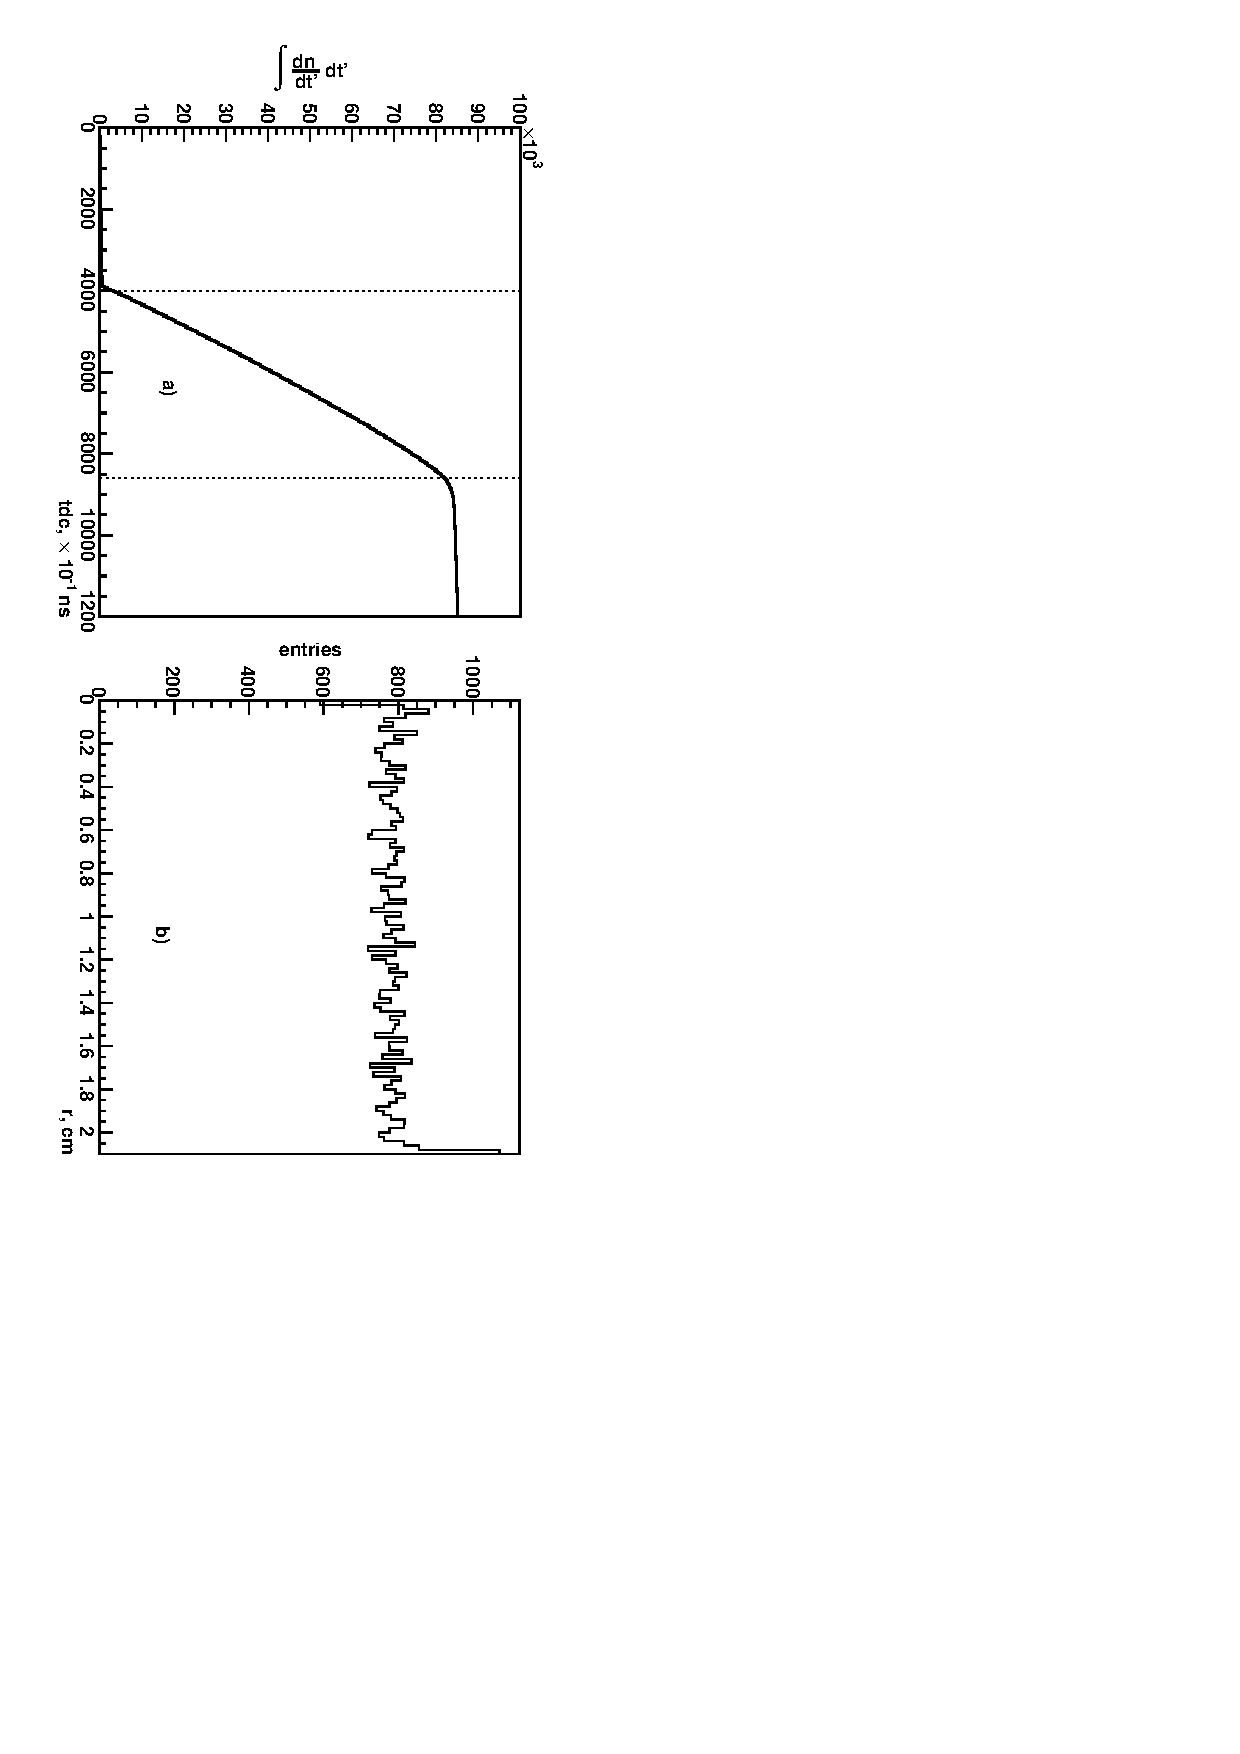
\includegraphics[angle=90,width=13.7cm]{t2r.pdf}
    \caption {Интегрированное a) время дрейфа $t$ проволочки из
      рис.~\ref{fig:tdc} и его преобразование b) в расстояние $r$ между
      сигнальной нитью и треком.}
    \label{fig:t2r}
  \end{center}
\end{figure}

Если предположить, что поток падающих частиц является равномерным,
а эффективность во всей области чувствительности проволочки постоянна,
то скорость дрейфа можно выразить как:
\[
v_{d}(t) = \frac{dr}{dt} = \frac{dr}{dn} \frac{dn}{dt} = const \frac{dn}{dt},
\qquad const = \frac{dr}{dn} = \frac{R}{N_{tot}},
\]
где $R$ длина дрейфового промежутка (21 мм), $N_{tot}$ полное число событий.
Таким образом, функцию преобразования времени дрейфа $t$ в расстояние $r$ можно
выразить как:
\[
r(t) = \int_{t_{min}}^{t_{max}} v_{d}(t') dt' = \frac{R}{N_{tot}} \int_{t_{min}}^{t_{max}} \frac{dn}{dt'}dt'.
\]
Заметим, что $r(t)$ отношение будет корректироваться (поправляться)
в~итеративном процессе автокалибровки.

\vspace* {0.5cm}
\begin{center} \bf{ПОИСК И РЕКОНСТРУКЦИЯ ТРЕКА} \end{center}

Поиск и реконструкция проекции трека происходит отдельно для каждого блока
одной плоскости дрейфовых камер. В зависимости от конкретной задачи, можно
программным путём, соединять (или разделять) блоки камер в один мультиблок.
В одном блоке (или мультиблоке) должно быть не менее трёх слоев сигнальных
проволочек, для возможности однозначного определения трека.

\begin{figure}[h]
  \begin{center}
    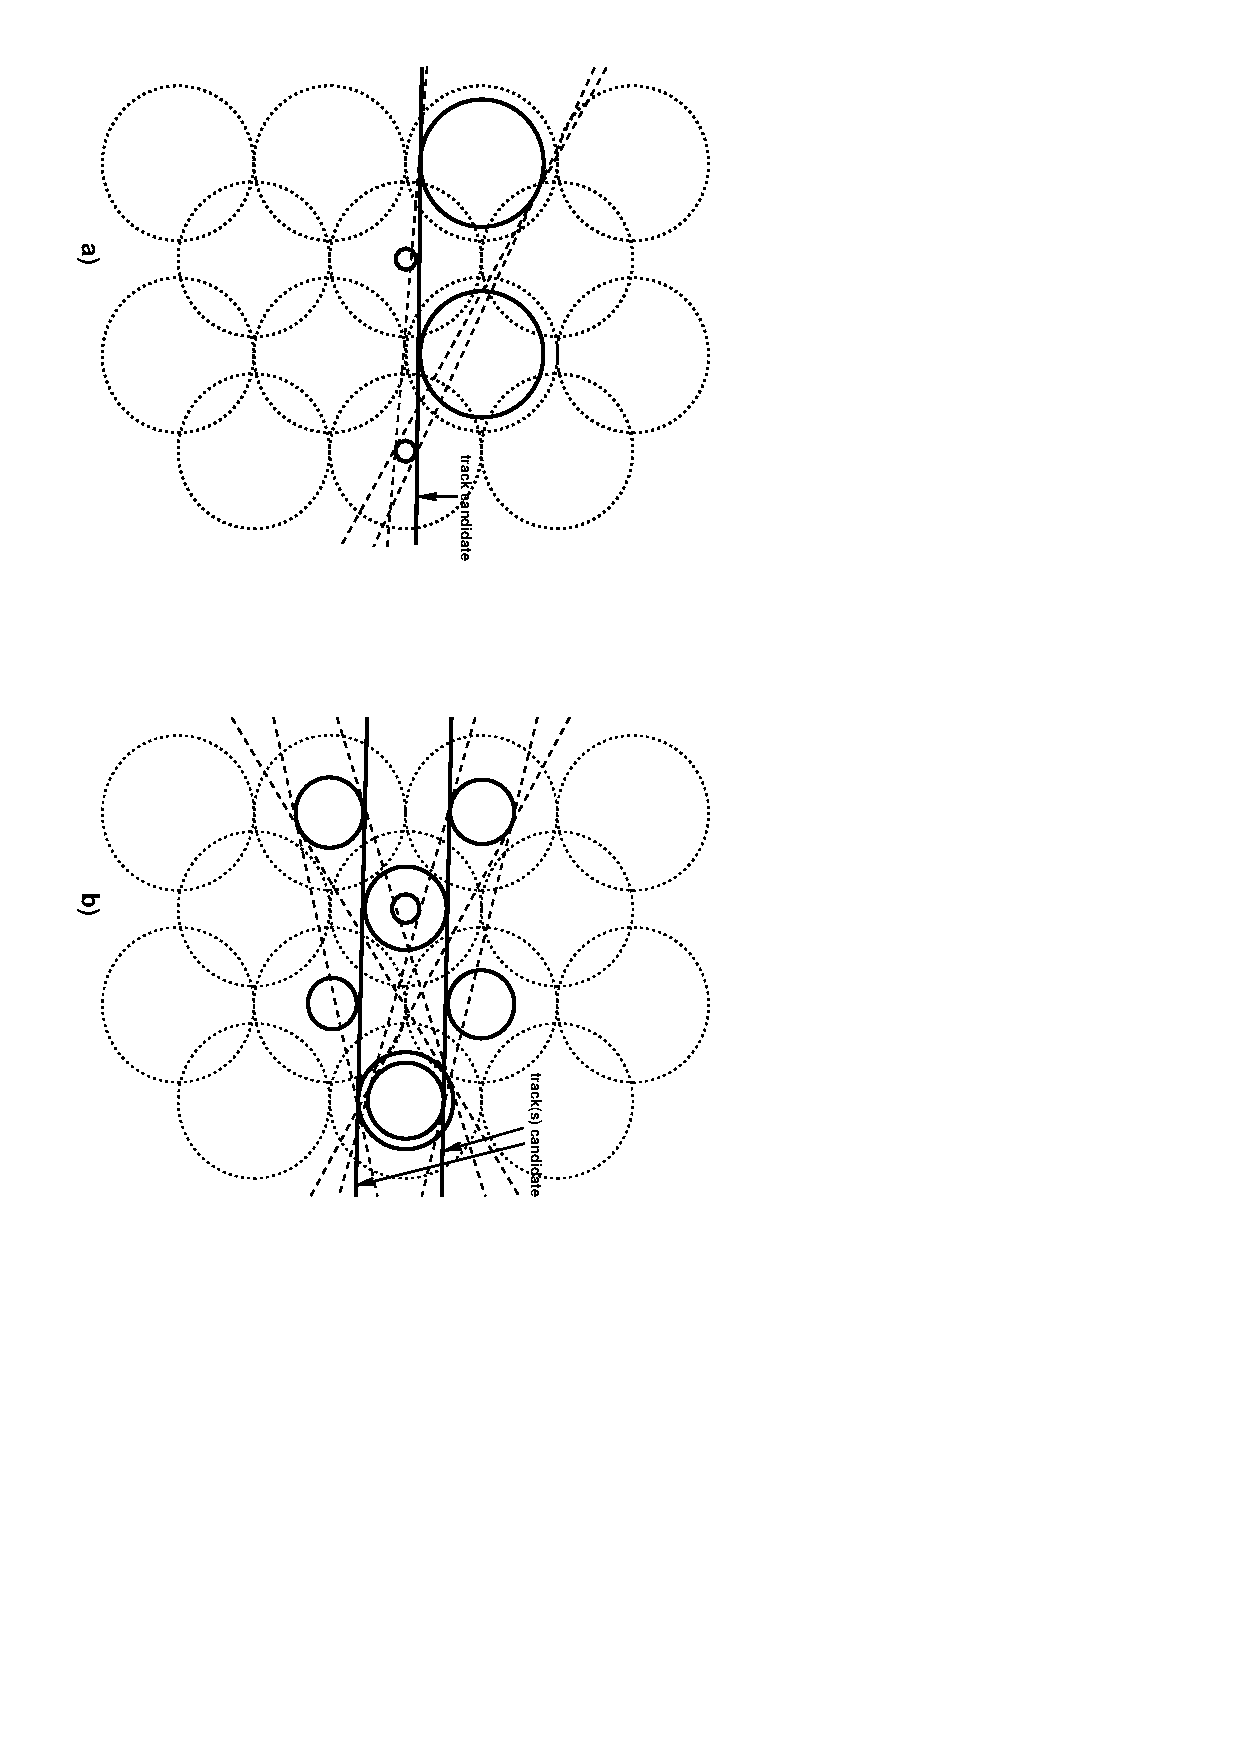
\includegraphics[angle=90,width=12.7cm]{typo_2events.pdf}
    \caption {Пример проекции одно a) и двух b) трекового события в одной
      плоскости блока первой дрейфовой камеры, состоящей из четырёх слоёв
      проволочек. Штриховые окружности представляют максимальную длину
      дрейфового промежутка, сплошные, расстояние трека от сигнальной нити.
      Для визуального изображения дрейфового промежутка используем окружности,
      центры которых проходят через сигнальные проволочки.}
    \label{fig:typo_event}
  \end{center}
\end{figure}

Последовательность поиска трека в упрощённом виде можно изложить следующим
образом:
\begin{itemize}
\item[а)]Поиск пары сработавших проволочек из разных слоев, имеющих наибольшее
  расстояние. Для пары окружностей, представляющих расстояние проекции трека
  от сигнальной нити, вычисляются параметры всех четырех касательных,
  рис.~\ref{fig:typo_event}а.
\item[б)]Для каждой касательной вычисляется её расстояние $d$ от окружности
  сработавших проволочек. Если расстояние больше, чем заданное минимальное
  $d > d_{min}$, то сработавшая проволочка отбрасывается (не считается).
  $d_{min}$ обычно на порядок больше, чем пространственное разрешение камеры.
\item[в)]Если число сработавших проволочек $N_{hits}$, удовлетворяющих
  предыдущему условию, для касательной не менее заданного $N_{min}$,
  $N_{hits} \geq N_{min}$, то касательная переходит в разряд кандидатов в трек.
  $N_{min}$ для нашего примера равно 4. Если кандидатов несколько, то
  оставляется тот, у которого сумма расстояний $d$ минимальна.
\item[г)] Производится реконструкция трека и возвращение к пункту а), поиску
  последующей пары. Сработавшие проволочки, которые входят в восстановленный
  трек, не удаляются и их можно использовать для поиска и реконструкции
  следующего трека, рис.~\ref{fig:typo_event}b.
\end{itemize}

Трек кандидат используется в процедуре реконструкции трека. Проекцию прямого
трека в плоскости перпендикулярной к проволочкам дрейфовой камеры можно
параметризовать как уравнение прямой:
\[
X = aZ + b
\]
с трековыми параметрами $a$ и $b$, рис.~\ref{fig:reco_scheme}.

\begin{figure}[h]
  \begin{center}
    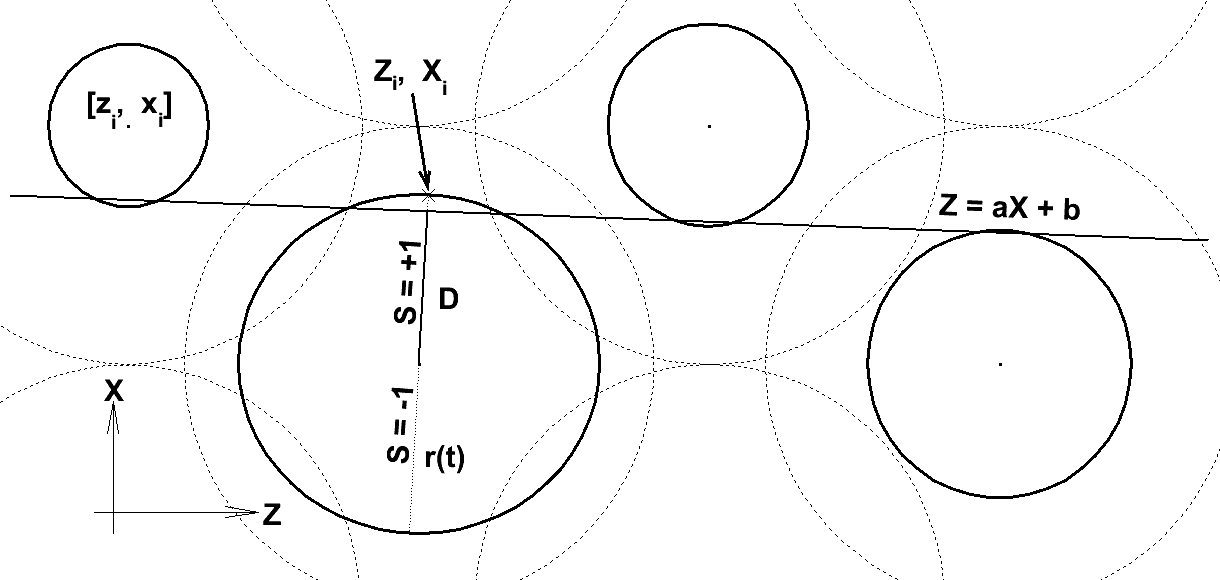
\includegraphics[angle=0,width=13.7cm]{reco_scheme.png}
    \caption {Определение параметров используемых при реконструкции трека.}
    \label{fig:reco_scheme}
  \end{center}
\end{figure}

Предположим, что трек имеет $N$ сработавших проволочек с координатами
$(z_{i}, x_{i})$ для $i = 1, \ldots N$. Тогда расстояние между треком и $i$-той
проволочкой можно выразит как:
\[
D_{i} = \frac{|a z_{i} - x_{i} + b|}{\sqrt{1 + a^{2}}}.
\]
Задача реконструкции трека состоит в~получении параметров прямой $a$ и $b$
путём минимизации $\chi^2$ функции:
\begin{equation}
\chi^2 = \frac{1}{N-2}\sum_{i=1}^{N} [|D_i| -S_ir_i]^2 =
\frac{1}{N-2}\sum_{i=1}^{N} \biggl[
\Big|\frac{az_i - x_i + b}{\sqrt{1 + a^2}}\Big| - S_ir_i\biggr]^2,
\end{equation}
где $S_i$ имеет в зависимости от положения трека относительно проволочки
значение $\pm{1}$ (смотри рис.~\ref{fig:reco_scheme}),
$r_i$~расстояние между треком и $i$-той проволочкой полученное из функции
преобразования времени дрейфа $t$ в~расстояние $r$. Величины параметров
$a$ и $b$ получаем решением двух дифференциальных уравнений
$\frac{\partial \chi^2}{\partial a} = 0$ и
$\frac{\partial \chi^2}{\partial b} = 0$, которые можно решить итеративно.
Уравнение (1) можно переписать следующим образом:
\begin{equation}
\chi^2 = \frac{1}{N-2}\sum_{i=1}^{N}
\biggl[\frac{aZ_i - X_i + b}{\sqrt{1 + a^2}}\biggr]^2,
\end{equation}
где координаты проволочек $(z_{i}, x_{i})$ заменяем координатами
$(Z_{i}, X_{i})$, которые вычисляются как:
\begin{equation}
Z_i = z_i - S_ir_i \frac{a_0}{\sqrt{1 + a_0^2}}, \qquad
X_i = x_i - S_ir_i \frac{1}{\sqrt{1 + a_0^2}}.
\end{equation}

Минимизируя $\chi^2$ функцию (уравнение 2), методом наименьших квадратов,
получаем значения трековых параметров $a$ и $b$. Величину $a_{0}$ в итеративном
процессе последовательно заменяем новым значением $a$. В~качестве начального
значение $a_{0}$ в уравнении (3) используем параметр $a$ из трека кандидата
(касательной). Для частиц падающих на камеру под небольшими углами можно
принять $a_{0} = 0$.

В среднем, после 2 -- 3 итераций параметры $a$ и $b$ практически не меняются
и если значение $\chi^2/ndf$  меньше заданного, то трек считаем восстановленным.

\vspace* {0.5cm}
\begin{center} \bf{АВТОКАЛИБРОВКА} \end{center}

Для реконструкции треков необходимо отношение между измеренным временем дрейфа
и его преобразованием в расстояние, поэтому, получение правильного $r(t)$
отношения, является одной из важнейших задач. Итеративную процедуру определения
$r(t)$ отношения с использованием трековой информации называем автокалибровкой
\cite{amelung:2004}.

Отметим, что $r(t)$ отношение полученное в процессе равномерного облучения
частицами дрейфового промежутка не учитывает неравномерность напряжённости
электрического поля вдоль траектории дрейфа электронов, а это, в свою очередь,
приводит к изменению величины скорости дрейфа и соответственно
к дифференциальной нелинейности $r(t)$ отношения. Это возможно в конструкции
используемых дрейфовых камер, где напряжённость электрического поля вдоль
траектории дрейфа задаётся резистивной сборкой, резисторы которой имеет разброс
в~несколько процентов.

Однако  можно предположить приблизительно одинаковые условия в~камере для
которой выполняется автокалибровка. При необходимости, можно программным путём
разделить камеры на меньшие или на группы проволочек, для которых предполагаем
те~же самые условия. Иногда поиск и реконструкция трека происходит в~одном
блоке (мульти-блоке) камер, но процедура автокалибровки проделывается для
каждой камеры отдельно.

На рис.~\ref{fig:multi_res} показана зависимость трекового остатка
$\triangle r$ (residual) от времени дрейфа в большой дрейфовой камере. Трековый
остаток, это разница между $r$, полученным преобразованием времени дрейфа $t$
в~расстояние, и~$D$, расстоянием восстановленного трека от проволочки
\[
\triangle r = r - |D|.
\]

\begin{figure}[h]
  \begin{center}
    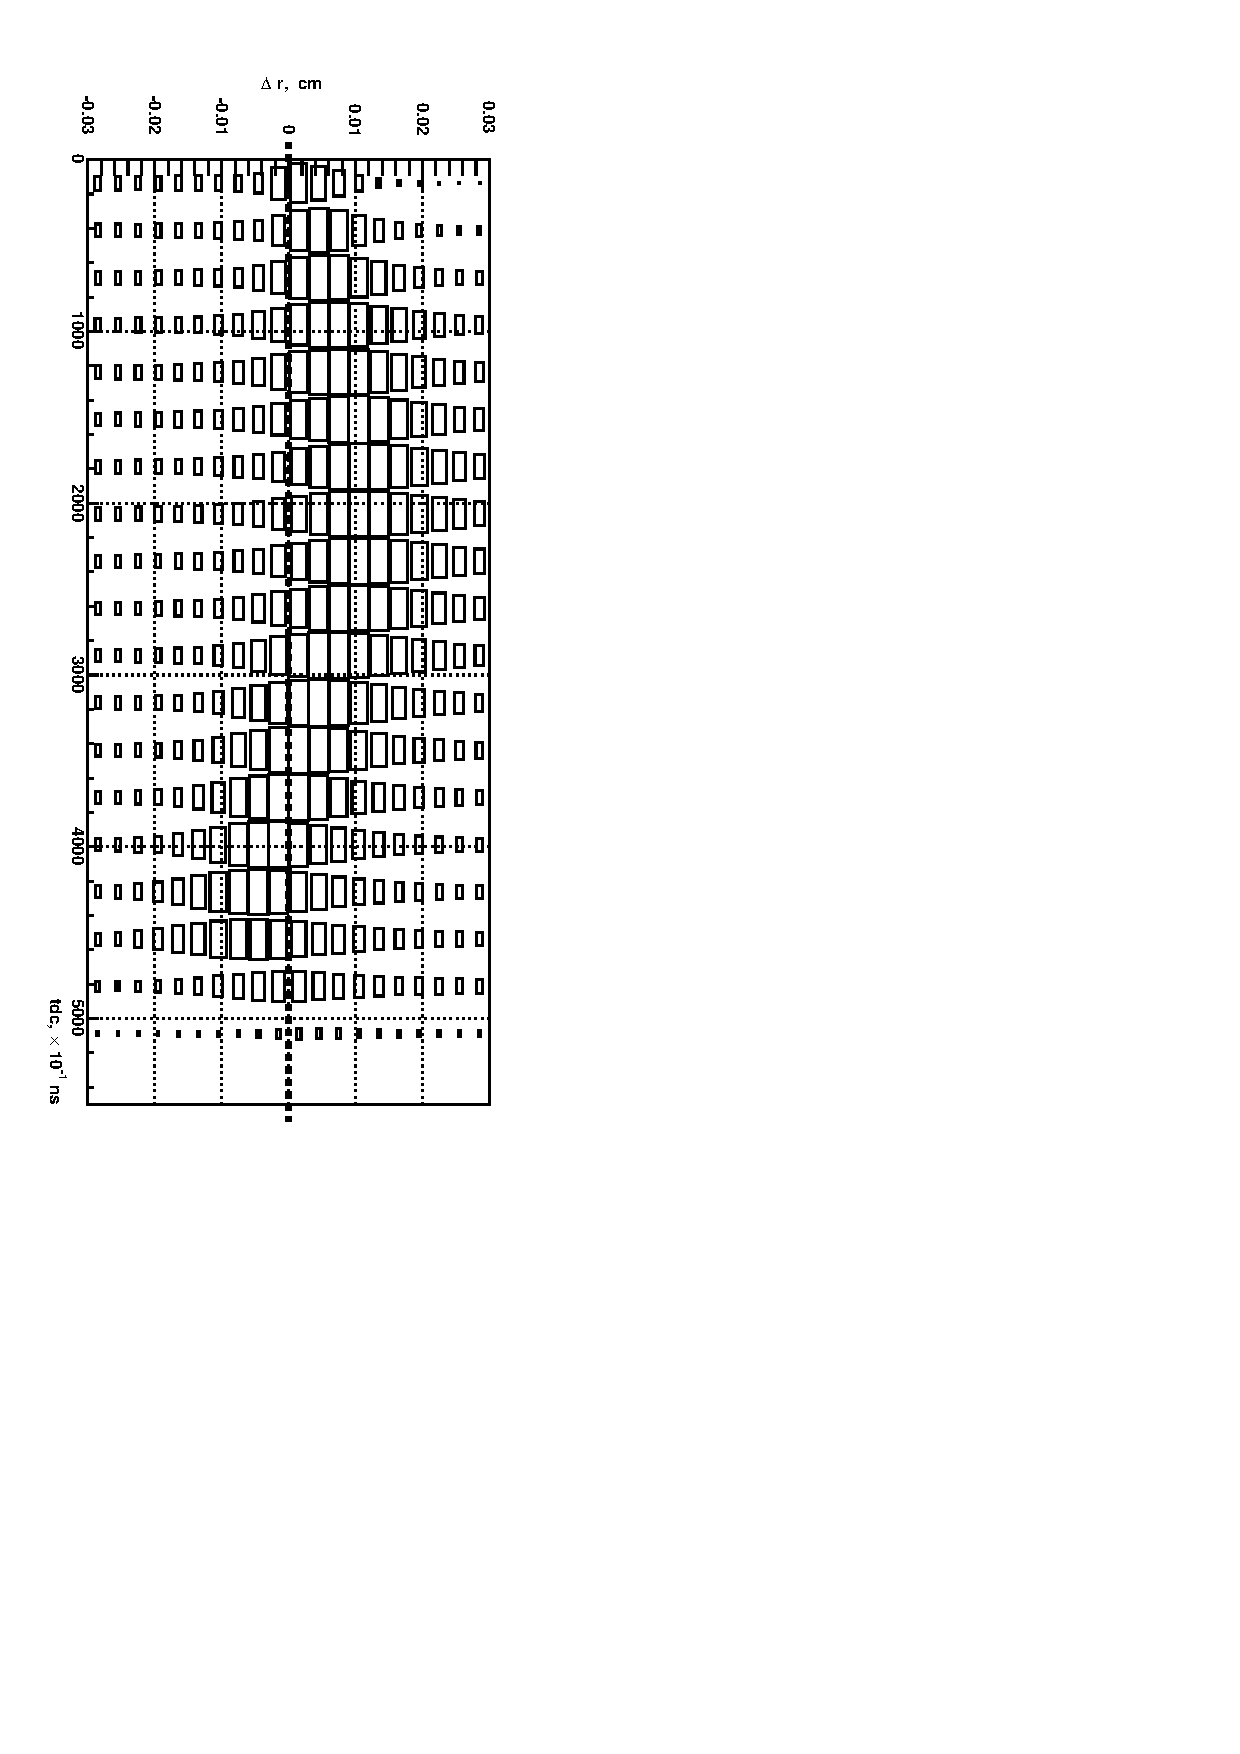
\includegraphics[angle=90,width=12.7cm]{multi_res_0.pdf}
    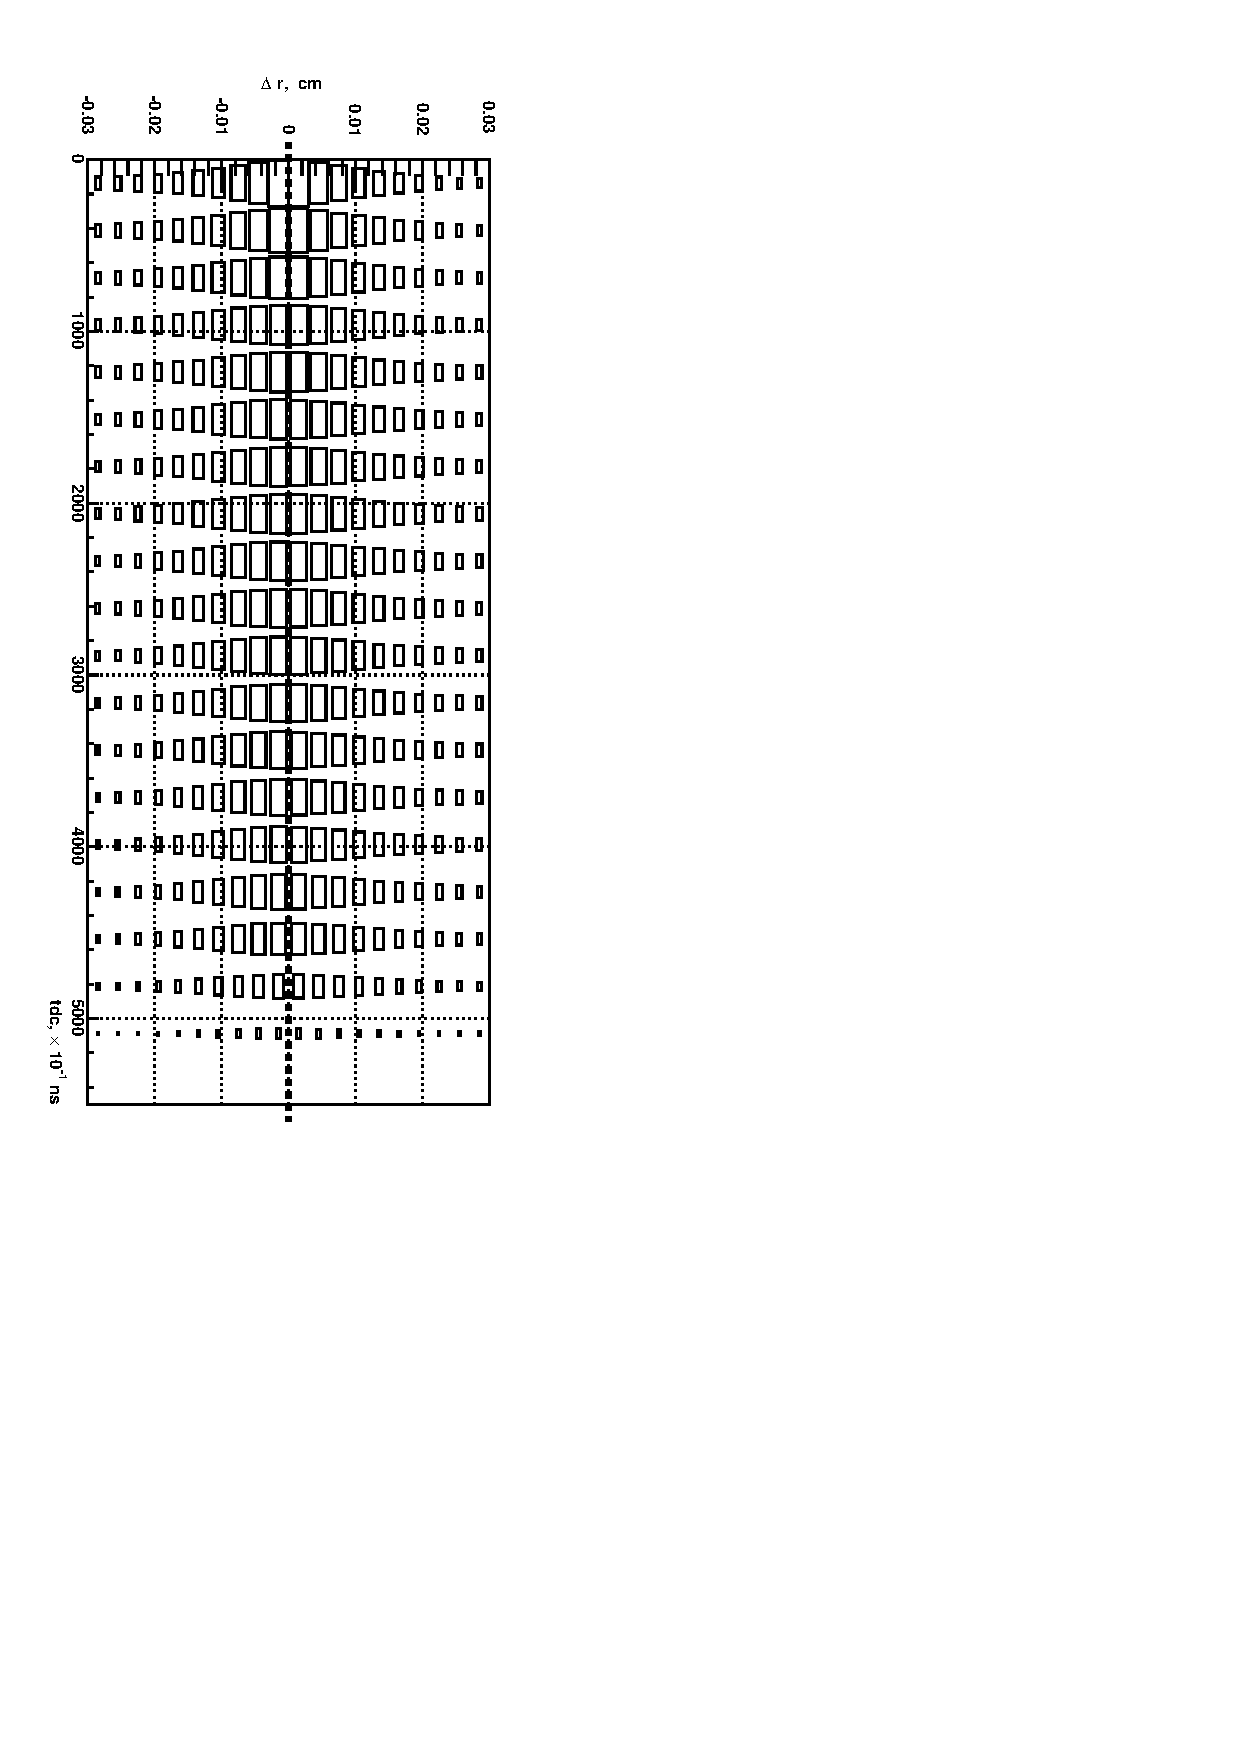
\includegraphics[angle=90,width=12.7cm]{multi_res_4.pdf}
    \caption {Зависимость распределения трекового остатка $\triangle r$ от
      времени дрейфа $t$ в плоскости XZ блока больших дрейфовых камер;
      a) для исходного $r(t)$ отношения (интегральное преобразование времени
      в расстояние), b) после окончательной, четвёртой итерации автокалибровки.
      Размер прямоугольника пропорционален числу событий.}
    \label{fig:multi_res}
  \end{center}
\end{figure}

Распределение трекового остатка (его ширина) в основном определяется
разрешением дрейфовой камеры. Тем не менее, $\triangle r$ можно использовать
при решении таких задач, как юстирование, сбалансирование проволочек в блоках
(мульти-блоках) камер относительно друг друга или для дополнительной оценки
минимального и максимального времени дрейфа ($T_{MIN}, T_{MAX}$). Ожидаемое
среднее значение остатка $\triangle r = 0$.

По горизонтальной оси двухмерной зависимости распределения $\triangle r$ от $t$
рис.~\ref{fig:multi_res}, отложено время дрейфа с шагом гистограммы 27.5 нс.
Шаг выбран так, чтобы получить необходимое число временных интервалов. В~нашем
примере оно равно 20. Для каждого временного интервала создаётся проекция
трекового остатка $\triangle r$. Полученное распределения остатка
аппроксимируется распределением Гаусса, среднее значение которого представляет
поправку $\delta_{i}$ к текущему $r(t)$ отношению в каждом $i$-том временном
интервале. Таким образом, получается новая, подправленная функция
преобразования времени дрейфа $t$ в расстояние~$r$, с которой вновь выполняется
реконструкция трека.

\begin{figure}[h]
  \begin{center}
    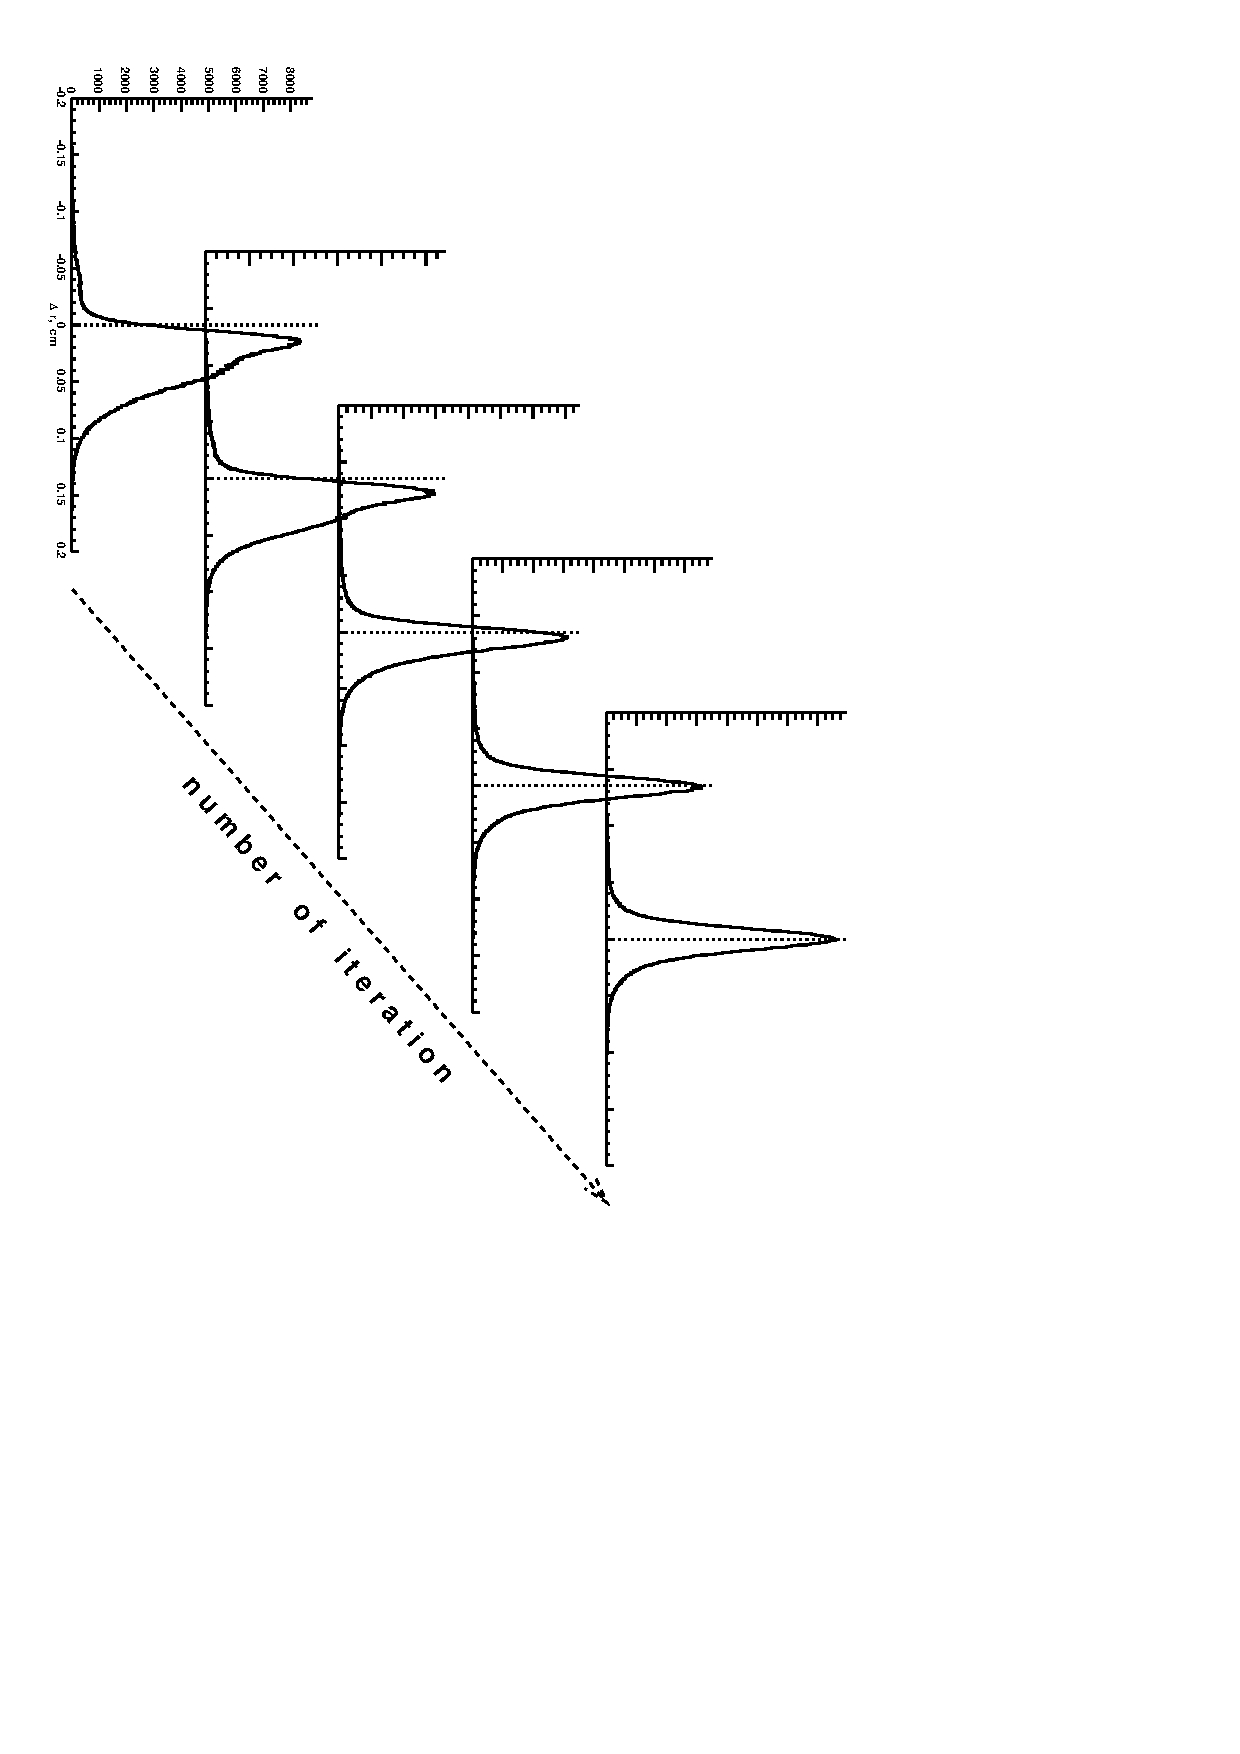
\includegraphics[angle=90,width=13.7cm]{res_iterative.pdf}
    \caption {Изменение распределения трекового остатка $\triangle r$
      в зависимости от номера итерации.}
    \label{fig:residual}
  \end{center}
\end{figure}

В каждом следующем шаге процедуры автокалибровки, $r(t)$ отношение поправляется
в зависимости от предыдущей итерации. Поиск и~реконструкция треков проводится
повторно до тех пор, пока значения поправок $\delta_{i}$ для всех временных
интервалов стабилизируются (близки к нулевым значениям). В нашем примере число
итерации равно 4 -- 5. Как меняется распределение трекового остатка
в зависимости от номера итерации показано на рис.~\ref{fig:residual}. Видно,
что с ростом номера итерации, трековый остаток стремиться к нулю, а ширина
распределения уменьшается.

Процесс автокалибровки выполняется только с однотрековыми событиями.
Желательно, чтобы угловой разброс треков не превышал $\sim$ 100 мрад.
Если диапазон наклонов треков проходящих через камеру большой, то итеративную
процедуру автокалибровки делаем отдельно для разных диапазонов углов наклона,
размером не больше $\sim$ 100 -- 150 мрад.

\begin{figure}[h]
  \begin{center}
    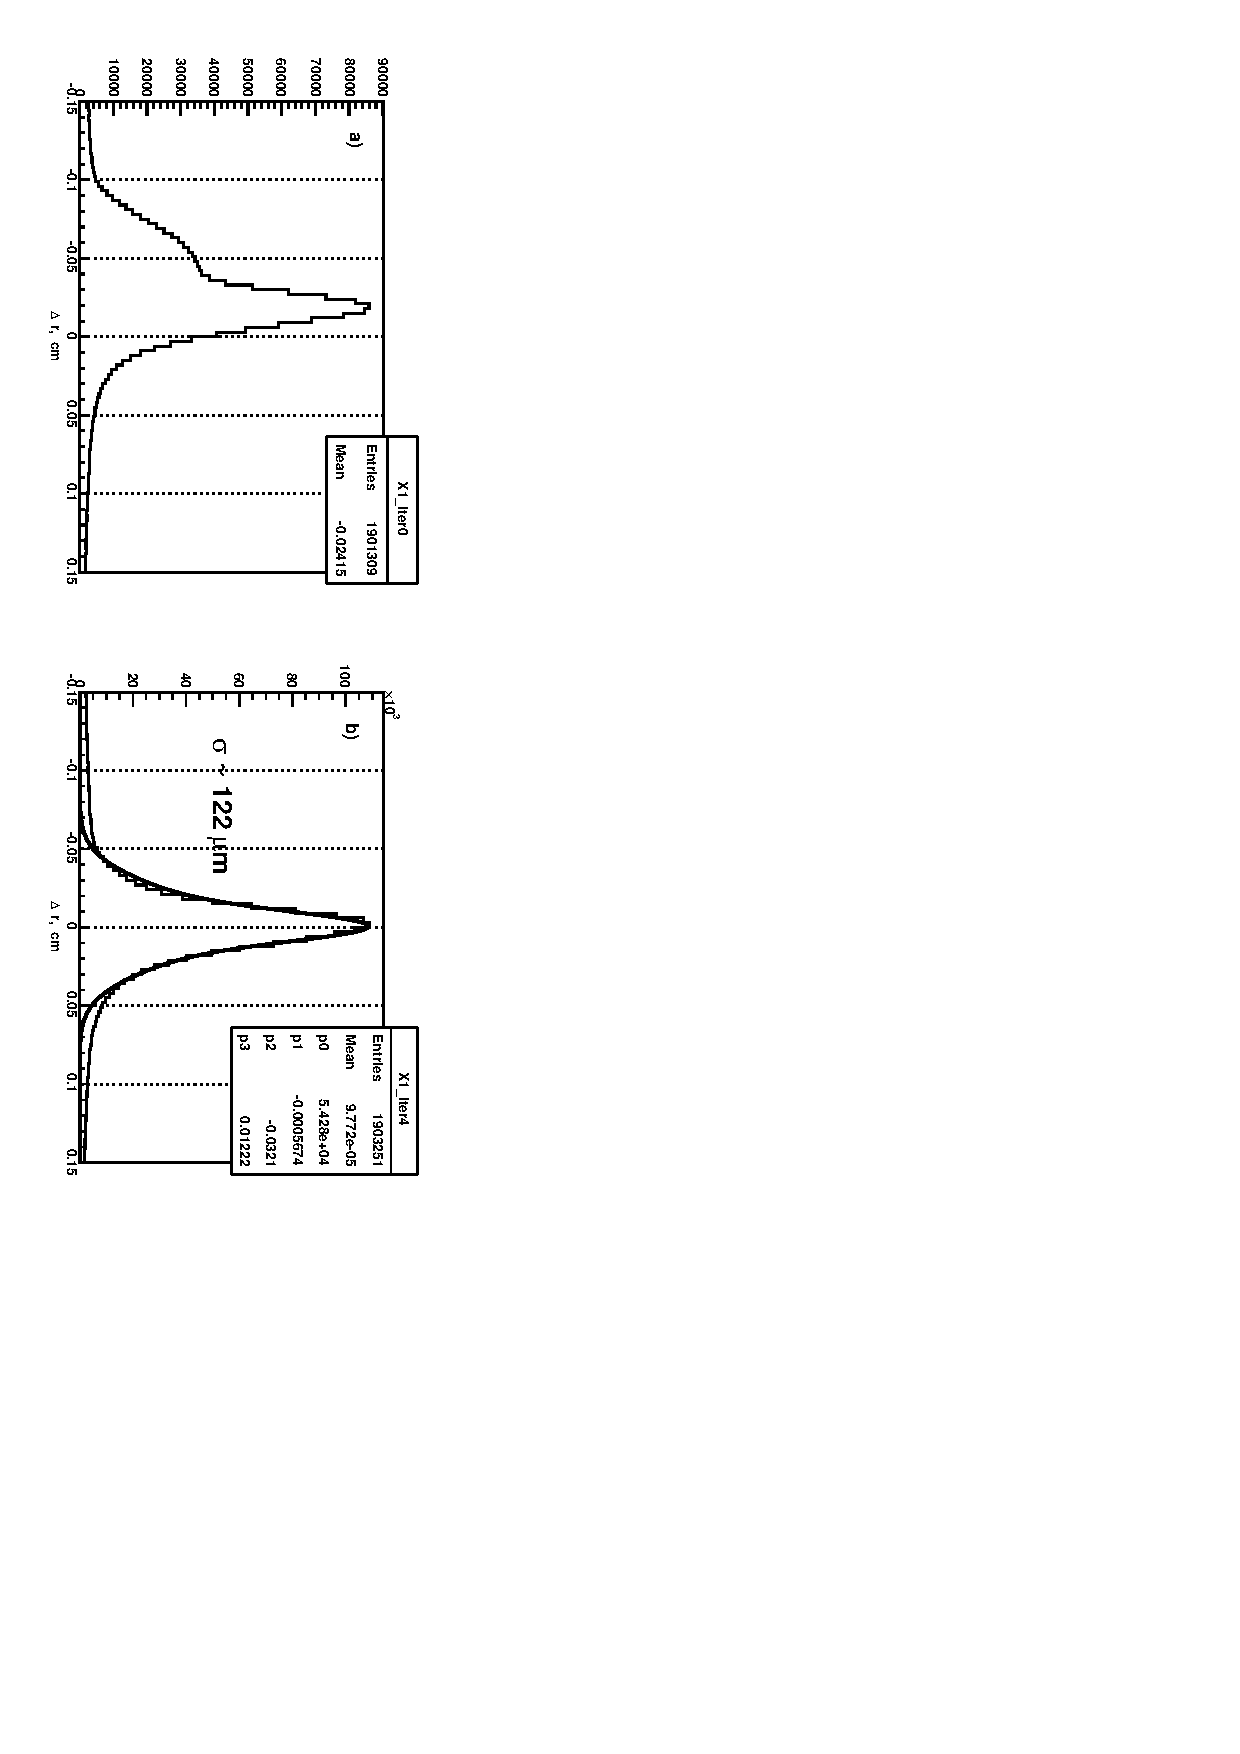
\includegraphics[angle=90,width=13.7cm]{reso_small.pdf}
    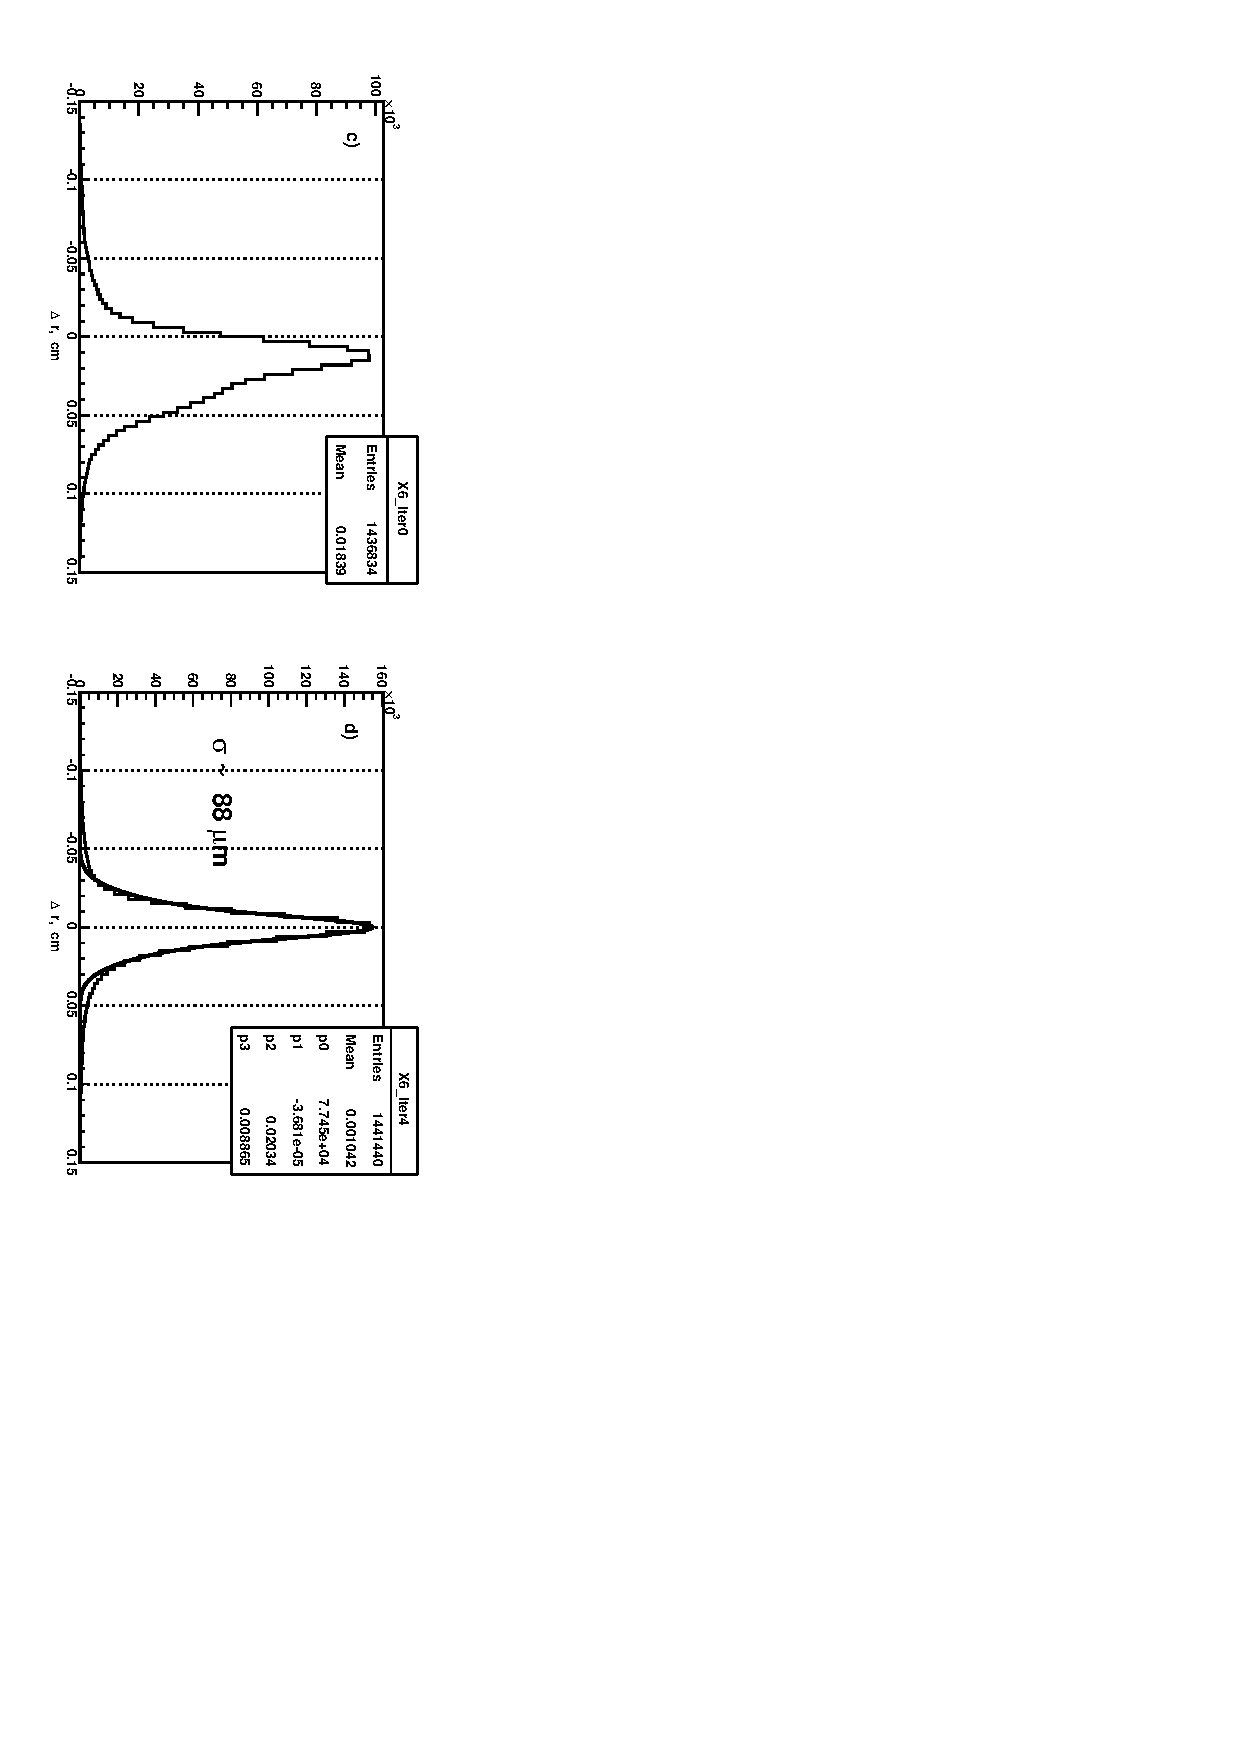
\includegraphics[angle=90,width=13.7cm]{reso_big.pdf}
    \caption {Распределения трекового остатка $\triangle r$ в XZ плоскости
      дрейфовой камеры D1 a), b) и камеры D6 c), d). Слева распределения
      с исходным интегральным $r(t)$ отношением, справа после финальной
      (четвёртой) итерации автокалибровки, фитированные двойным распределением
      Гаусса.}
    \label{fig:final_res}
  \end{center}
\end{figure}

Пространственное разрешение дрейфовой камеры определяется шириной распределения
трекового остатка данной камеры. Для вычисления разрешения $\sigma$
использовалась аппроксимация двойным распределением Гаусса,
рис.~\ref{fig:final_res}. Пространственное разрешении $\sigma$ дрейфовых камер,
используемых на установке СТРЕЛА, лежит в диапазоне $\sim 90 - 120$ $\mu m$.
Влиянием многократного рассеяния (дейтроны с импульсом  3.5 ГэВ/с) на
разрешение можно пренебречь.

\vspace* {0.5cm}
\begin{center} \bf{ЗАКЛЮЧЕНИЕ} \end{center}

Результаты работы можно сформулировать следующим образом:
\begin{itemize}
\item Проверена работа всех блоков дрейфовых камер экспериментальной
  установки СТРЕЛА.
\item Создан и протестирован алгоритм для поиска и реконструкции треков
  в дрейфовых камерах (или трубках).
\item Исходный код программы написан полностью в C++ с использованием ROOT
  библиотек (универсальность, модульность программы).
\item Итеративная процедура автокалибровки улучшает величину пространственного
  разрешение камер.
\item Полученные характеристики трековых детекторов позволяют осуществить
  исследования зарядово-обменных процессов в взаимодействиях дейтронов
  с протонами на установке СТРЕЛА.
\end{itemize}

Данная работа выполнена при поддержке гранта Словакии \No 1/4010/07.



%%% Local Variables:
%%% TeX-master: "preprint"
%%% End:


\begin{thebibliography}{99}
\bibitem{cejp:2008}
  \emph{Glagolev V. V. et al. //} Cent. Eur. J. Phys. 2008. V. 6(4). P.781-785
\bibitem{strela:web}
  \emph{http://strela.jinr.ru}
\bibitem{filatova:1977}
  \emph{Filatova N. A. et al. //} Nucl. Instr. and Meth. 1977. V. 143. P.17-28
\bibitem{vodopianov:1975}
  \emph{Водопьянов А. С. и др.//} препринт ОИЯИ P13-9351. Дубна, 1975.
\bibitem{vodopianov:1983}
  \emph{Водопьянов А. С. и др.//} препринт ОИЯИ P1-83-12. Дубна, 1983.
\bibitem{hera:web}
  http://www-hera-b.desy.de/subgroup/detector/tracker/outer/
\bibitem{erfc:web}
  http://root.cern.ch/root/html/TMath.html\#TMath:Erfc
\bibitem{peshenov:1986}
  \emph{В. Пешехонов //} Физ. элем. частиц и атом. ядра. 1986. Т. 17(5).
  с.1030-1078
\bibitem{amelung:2004}
  \emph{Ch. Amelung //} ATLAS Muon Note, ATL-MUON-2004-020, 2004.
\end{thebibliography}

\clearpage % -*- mode: LaTeX; coding: utf-8; -*-

\thispagestyle{empty}

\noindent
Мушински Я. и др.\\
Поиск и реконструкция трека в дрейфовых камерах на установке Стрела \\

Изучение характеристик дрейфовых камер на экспериментальной установке СТРЕЛА
было проведено на пучке ускорительного комплекса Нуклотрона ЛФВЭ ОИЯИ.
Приводится описание метода поиска и реконструкции трека. Применение дрейфовых
камер требует корректного определения $r(t)$ соотношения с помощью итеративной
процедуры автокалибровки. Знание характеристик время-координатной зависимости
позволило улучшить точность пространственного разрешения дрейфовых камер
установки СТРЕЛА. \\

Работа выполнена в Лаборатории физики высоких энергий им. В. И.~Векслера и
А. М.~Балдина ОИЯИ.



%%% Local Variables:
%%% mode: latex
%%% TeX-master: "preprint"
%%% End:

\clearpage % -*- mode: LaTeX; coding: utf-8; -*-

\thispagestyle{empty}

\noindent
Mu\v{s}insk\'{y} J. et al.\\
Searching and reconstruction of the track in the drift chambers of the
STRELA setup. \\

Investigation of the drift chambers of the STRELA setup was performed in the
beam of the Nuclotron accelerator complex of the JINR Laboratory of High Energy
Physics. The descriptions of track-finding and reconstruction methods are
given. Using of drift chamber in experiment needs the correct determination
of the distance-to-drift time relation $r(t)$. This relation is auto calibrated
by an iterative procedure. Knowledge of the correct relation between the time
and space scales allows improving the accuracy of coordinate resolution of the
STRELA drift chambers. \\

The work was done in the Veksler and Baldin Laboratory of High Energy Physics
of the Joint Institute for Nuclear Research.



%%% Local Variables:
%%% mode: latex
%%% TeX-master: "preprint"
%%% End:


\end{document}



%%% Local Variables:
%%% TeX-master: t
%%% End:
